\documentclass{beamer}

\usepackage{amsmath}
\usepackage{textcomp}
\usepackage{listings}
\usepackage{lmodern}
\usepackage{hyperref}
\usepackage[T1]{fontenc}


\lstset{
    language=[latex]tex,
    breaklines=true}

\usetheme{Madrid}

\setbeamertemplate{caption}{\raggedright\insertcaption\par}

\title[Committee Meeting 1]{First Committee Meeting}
\subtitle{Progress Report}
\author{Jason Balaci}

\institute{McMaster University}
\date{Oct. $21^{st}$, 2021}

\AtBeginSection[]
{
  \begin{frame}
    \frametitle{Table of Contents}
    \tableofcontents[currentsection]
  \end{frame}
}

\begin{document}

%%%%%%%%%%%%%%%%%%%%%%%%%%%%%%%%%%%%%%%%%%%%%%%%%%%%%%%%%%%%%%%%%%%%%%%%%%%%%%%
%% TITLE PAGE
%%%%%%%%%%%%%%%%%%%%%%%%%%%%%%%%%%%%%%%%%%%%%%%%%%%%%%%%%%%%%%%%%%%%%%%%%%%%%%%
\frame{\titlepage}

%%%%%%%%%%%%%%%%%%%%%%%%%%%%%%%%%%%%%%%%%%%%%%%%%%%%%%%%%%%%%%%%%%%%%%%%%%%%%%%
%% TABLE OF CONTENTS
%%%%%%%%%%%%%%%%%%%%%%%%%%%%%%%%%%%%%%%%%%%%%%%%%%%%%%%%%%%%%%%%%%%%%%%%%%%%%%%

\begin{frame}
\frametitle{Table of Contents}
\tableofcontents
\end{frame}

%%%%%%%%%%%%%%%%%%%%%%%%%%%%%%%%%%%%%%%%%%%%%%%%%%%%%%%%%%%%%%%%%%%%%%%%%%%%%%%
%% INTRODUCTION
%%%%%%%%%%%%%%%%%%%%%%%%%%%%%%%%%%%%%%%%%%%%%%%%%%%%%%%%%%%%%%%%%%%%%%%%%%%%%%%
\section{Introduction}

% TODO: How personal do I want to get?
% TODO: Mention 3D printing or no?

\begin{frame}
    \frametitle{Who am I?}
    \begin{columns}[T,onlytextwidth]
        \begin{column}{.5\textwidth}
            \begin{minipage}{\textwidth}
                \begin{itemize}
                    \item<2-> I am \textbf{Jason Balaci}
                    \item<3-> Graduate of \emph{McMaster University}, holding...
                        \begin{itemize}
                            \item<4-> Hons. Actuarial and Financial Mathematics (B.Sc.)
                            \item<5-> Minor in Computer Science
                        \end{itemize}
                    \item<6-> Currently pursuing a thesis-based Master's of Computer Science (M.Sc) at \emph{McMaster University}, under the supervision of \textbf{Dr. Jacques Carette}
                \end{itemize}
            \end{minipage}
        \end{column}
        \begin{column}{.45\textwidth}<2->
            \begin{figure}
                
\includegraphics[width=.8\textwidth]{assets/me.jpeg}
                \caption{Me, Fall 2019}
            \end{figure}
        \end{column}
    \end{columns}
\end{frame}

\begin{frame}
    \frametitle{Overview of Progression Towards C.S. M.Sc.}
    \framesubtitle{Course-related progression}
    \begin{itemize}
        \item<1-> I'm required to complete\footnotemark[1]:
            \begin{itemize}
                \item<2-> One (1) ``Software'' course
                \item<3-> Either of:
                    \begin{itemize}
                        \item<4-> Two ``Theory'' courses, and one ``Systems'' course
                        \item<4-> One ``Theory'' course, and two ``Systems'' courses
                    \end{itemize}
            \end{itemize}
        \item<5-> I've completed:
            \begin{itemize}
                \item<6-> CAS 701 ``Logic \& Discrete Mathematics'' - Theory course, Fall 2020
                \item<6-> CAS 761 ``Generative Programming'' - Software course, Fall 2020
                \item<6-> CAS 763 ``Certified Programming with Dependent Types'' - Theory \& Software course, Winter 2021
                \item<6-> COMPSCI 6TB3 ``Syntax-Based Tools and Compilers'' - Systems course, Winter 2021
            \end{itemize}
        \item<7-> Together, the courses completed satisfies the ``Courses Requirement'' as mentioned in the academic calendar\footnotemark[1] and the ``Regulations for the Computer Science M.Sc. Program'' document\footnotemark[2].
    \end{itemize}

    \footnotetext[1]{\tiny\url{https://academiccalendars.romcmaster.ca/preview_program.php?catoid=45&poid=23470&returnto=9166}}
    \footnotetext[2]{\tiny\url{http://www.cas.mcmaster.ca/cas/0files/reg_master_cs_2019a.pdf}}
\end{frame}

\begin{frame}
    \frametitle{Overview of Progression Towards C.S. M.Sc.}
    \framesubtitle{Thesis/research-related Progression}
    \begin{itemize}
        \item<1-> Conducted ``full-time'' research for at least 1 full semester (Spring/Summer 2021), and ``part-time'' research during courses.
        \item<2-> Continuing to research ``full-time''.
        \item<3-> Attended a thesis defence to learn about what to expect from a thesis defence meeting (and learn about their research).
        \item<4-> Supervisory committee is formed, and we're currently having our first supervisory committee.
            \begin{itemize}
                \item \emph{Supervisor}: Dr. Jacques Carette
                \item Dr. Spencer Smith
                \item Dr. Wolfram Kahl
            \end{itemize}
    \end{itemize}
\end{frame}

%%%%%%%%%%%%%%%%%%%%%%%%%%%%%%%%%%%%%%%%%%%%%%%%%%%%%%%%%%%%%%%%%%%%%%%%%%%%%%%
%% PROJECT
%%%%%%%%%%%%%%%%%%%%%%%%%%%%%%%%%%%%%%%%%%%%%%%%%%%%%%%%%%%%%%%%%%%%%%%%%%%%%%%

\section{Project}
\subsection{Drasil}

\begin{frame}
    \frametitle{Preface}
    \framesubtitle{What is Drasil?}
    \begin{columns}[T,onlytextwidth]
        \begin{column}{.5\textwidth}
            Drasil...
            \newline \newline
            \begin{minipage}{\textwidth}
                \begin{itemize}
                    \item<1-> is managed by Dr. Carette \& Dr. Smith.
                    \item<2-> originates from the work of Dan Szymczak.
                        \begin{itemize}
                            \item<3-> Originally focused on scientific software (\emph{Literate Scientific Software}).
                            \item<4-> Focus shifted into...
                        \end{itemize}
                    \item<5-> tries to ``Generate All The Things''...
                    \begin{itemize}
                        \item<6-> with a focus on research software.
                    \end{itemize}
                \end{itemize}
            \end{minipage}
        \end{column}
        \begin{column}{.45\textwidth}
            \begin{figure}
                
\includegraphics[width=.8\textwidth]{assets/drasil-logo.png}
                \caption{Drasil's Logo \tiny\cite{Drasil2021}\cite{YggdrasilWiki2021}} % TODO: Origin of file
            \end{figure}
        \end{column}
    \end{columns}
\end{frame}

\begin{frame}
    \frametitle{Drasil}
    \framesubtitle{``Generate All The Things!''}
    
    \begin{itemize}
        \item TODO: here!
% TODO: ``Generate All The Things!'' is a beautifully appropriate tagline for Drasil
%       for a few reasons:
%                  1. What are ``Things''? One may only think of ``Things'' as far as their knowledge and understanding allows them! You wouldn't be able to think of things without some sort of basis/constructive understanding/methodology to _get_ there, you can't _think of random phenomena_ (that's why they're phenomena).
    \end{itemize}
\end{frame}

% TODO: Currently contained examples...
\begin{frame}
    \frametitle{What does Drasil currently support?}
    \begin{itemize}
        \item<2-> Drasil currenty contains a significant amount of Physics-related knowledge.
        \item<3-> Current case studies include:
            \begin{itemize}
                \item<4-> \textbf{GlassBR} - Predicting whether or not a glass slab is likely to resist a specified blast.
                \item<5-> \textbf{Single Pendulum} - Calculating the motion of a single pendulum.
                \item<6-> \textbf{Double Pendulum} - Calculating the motion of a double pendulum.
                \item<7-> \textbf{Game Physics} - 
                \item<8-> \textbf{Proportional Derivative Controller (PDController)} - 
                \item<9-> \textbf{Solar Water Heating System (SWHS)} - 
                \item<10-> \textbf{SWHS without Phase Change Material (NoPCM)} - 
                \item<11-> \textbf{Projectile} - 
                \item<12-> \textbf{Slope Stability Analysis (SSP)} - 
                \item<13-> \textbf{Heat Transfer Coefficients between Fuel and Cladding in Fuel Rods (HGHC)} - Examining the heat transfer coefficients related to clad.
            \end{itemize}
    \end{itemize}
\end{frame}

\begin{frame}
    \frametitle{Example: GlassBR}
    \begin{figure}
        \center
        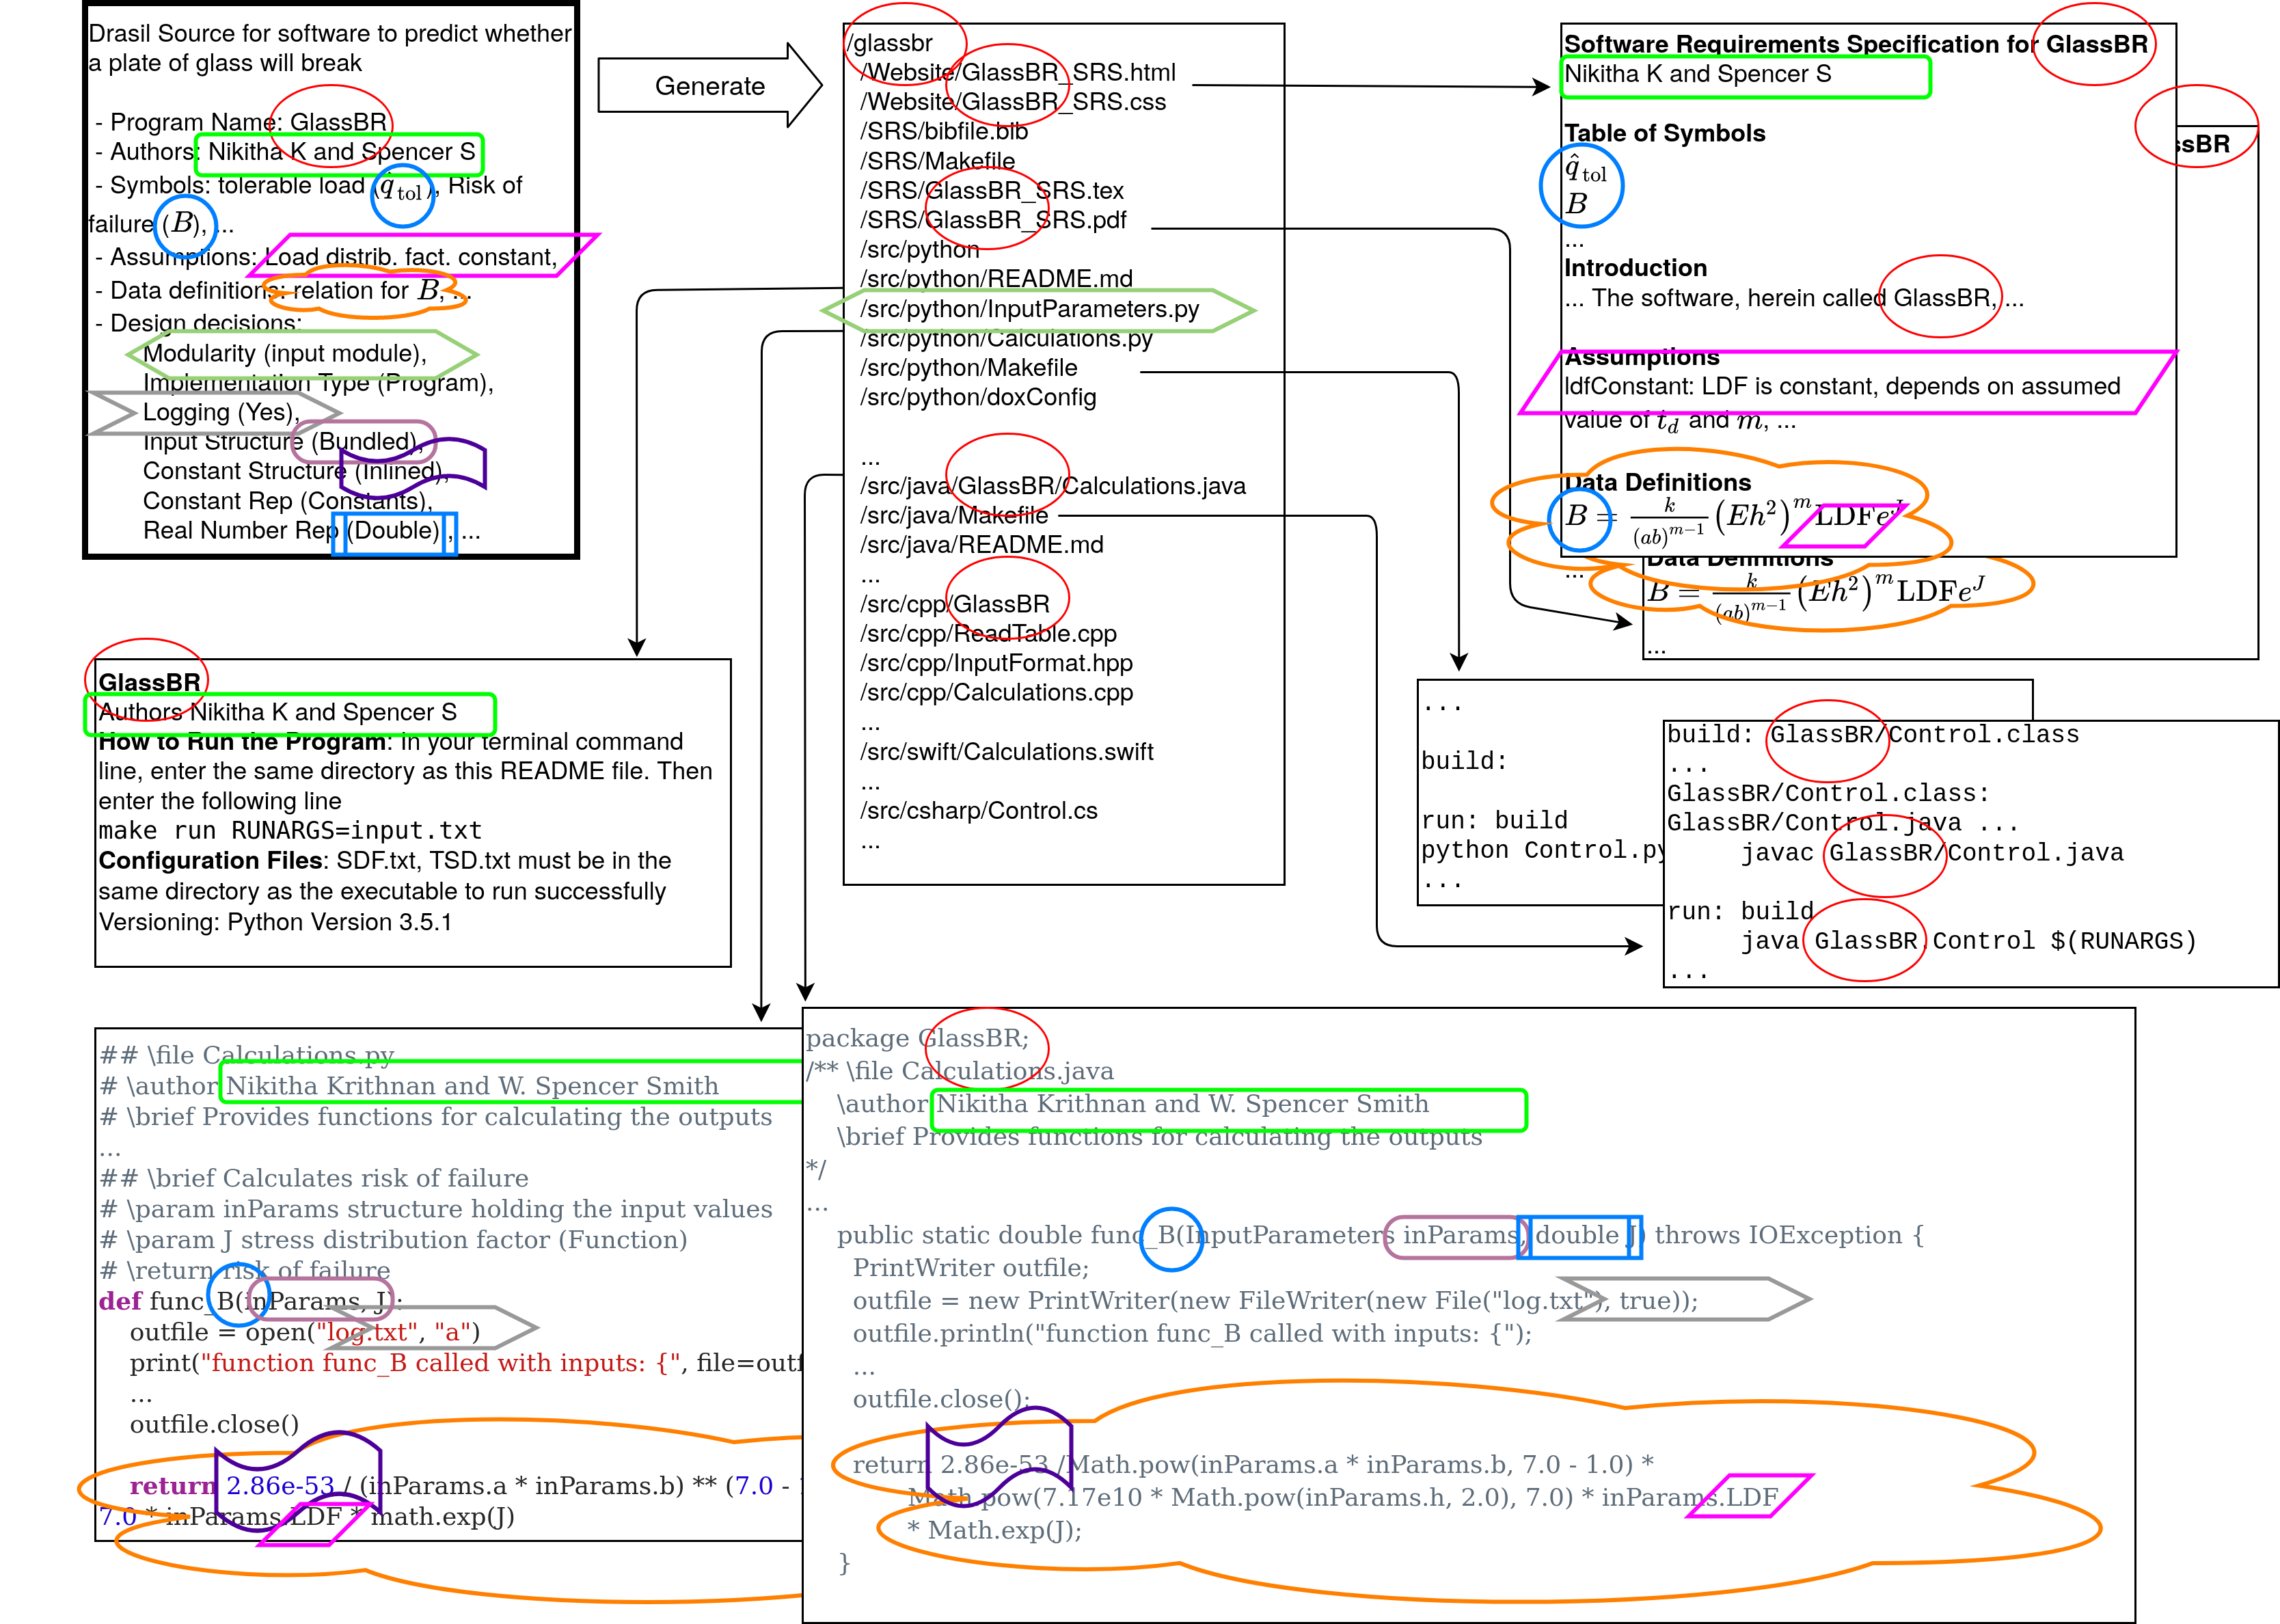
\includegraphics[width=0.75\textwidth]{assets/DrasilSupportsChange.png}
        \caption{Figure created by Dr. Spencer Smith.}
        \label{fig:glassbr}
    \end{figure}
\end{frame}

\begin{frame}
    \frametitle{Which case studies currently generate code?}
    \begin{alertblock}{\footnotesize Not all case studies generate code yet!}<2->
        {\tiny Some are a work-in-progress, and some require more infrastructure to enable it.}
    \end{alertblock}
    
\end{frame}

% TODO: What's stopping the non-code-generating examples from having workable generable code?
\begin{frame}
    \frametitle{}
    
\end{frame}

\begin{frame}
    \frametitle{Where will I be contributing?}
    %% TODO: What I will be contributing
\end{frame}

\subsection{Goal \#1: Typed Expression Language}
%% TODO: Problem?
%% TODO: What is a good ``solution''?
%% TODO: Current project status?

\subsection{Goal \#2: Model Discrimination -- ``ModelKinds''}
%% TODO: Problem?
%% TODO: What is a good ``solution''?
%% TODO: Current project status?

%%%%%%%%%%%%%%%%%%%%%%%%%%%%%%%%%%%%%%%%%%%%%%%%%%%%%%%%%%%%%%%%%%%%%%%%%%%%%%%
%% REFERENCES
%%%%%%%%%%%%%%%%%%%%%%%%%%%%%%%%%%%%%%%%%%%%%%%%%%%%%%%%%%%%%%%%%%%%%%%%%%%%%%%

\begin{frame}
    \center
    \huge{Fin.}\\
    \normalsize{Thank you!}
\end{frame}

%%%%%%%%%%%%%%%%%%%%%%%%%%%%%%%%%%%%%%%%%%%%%%%%%%%%%%%%%%%%%%%%%%%%%%%%%%%%%%%
%% REFERENCES
%%%%%%%%%%%%%%%%%%%%%%%%%%%%%%%%%%%%%%%%%%%%%%%%%%%%%%%%%%%%%%%%%%%%%%%%%%%%%%%

\section{References}

\begin{frame}[allowframebreaks]
    \frametitle{References}

    \bibliography{references}
    \bibliographystyle{amsalpha}
\end{frame}


\end{document}
